\chapter{الدوال (\textenglish{Functions})}

ننتهي من الجزء الأول من الكتاب (المبادئ) بهذها المفهوم المهم الذي يتكلّم عن الدوال في لغة
\textenglish{C}.
كل البرامج في لغة  
\textenglish{C}
ترتكز على المبدأ الذي سأشرحه في هذا الفصل.

سوف نتعلم هيكلة برامجنا وتقسيمها لعدة أجزاء، تقريباً كما لو كنّا نلعب لعبة
\textenglish{Lego}.\\
البرامج الكبيرة في لغة 
\textenglish{C}
ماهي إلا تجميعات لأجزاء صغيرة من الشفرات المصدرية، و هذه الأجزاء هي بالضبط ما نسمّيه \dots بالدوال !

\section{إنشاء و استدعاء دالة}

رأينا في الفصول السابقة بأن برامج الـ\textenglish{C}
تبدأ بدالة تدعى 
\InlineCode{main}.
لقد أعطيتك مخططاً تلخيصيّاً لتذكيرك ببعض الكلمات المفتاحية :

\begin{figure}[H]
	\centering
	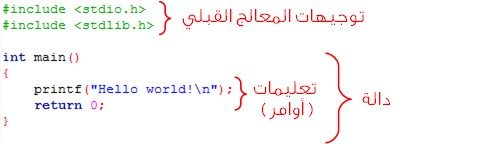
\includegraphics[width=0.8\textwidth]{Chapter_I-9_main}
\end{figure}

في الأعلى، نجد توجيهات المعالج القبلي (اسم معقد سأرجع لشرحه في وقت لاحق). من السهل التعرّف على هذه التوجيهات : هي تبدأ بإشارة 
\InlineCode{\#}
و هي غالباً توضع في أعلى الملف المصدري.

لقد قلت لك بأن البرنامج في الـ\textenglish{C}
يبدأ بالدالة
\InlineCode{main}.
 أؤكد لك، هذا صحيح ! إلا أننا في هذه الحالة بقينا داخل الدالة 
\InlineCode{main}
و لم نخرج أبداً منها. أعد قراءة الشفرات المصدرية في الدروس السابقة و سترى : لقد بقينا دائما داخل الحاضنتين الخاصتين بالدالة الرئيسية.

\begin{question}
حسنا، هل من السيء فعل ذلك ؟
\end{question}

لا، هذا ليس "سيئا". لكن ذلك خلاف ما يفعله المبرمجون بلغة
\textenglish{C}
حقيقة.\\
بل و إن كل البرامج تقريباً لا تكون مكتوبة فقط داخل  حاضنتي الدالة 
\InlineCode{main}.
لحدّ الآن كانت البرامج التي نكتبها صغيرة و لهذا فهي لم تطرح أي مشكل، لكن تخيّل معي برامج ضخمة تحتوي على آلاف الأسطر من الشفرة المصدرية ! لو كانت كلّ الأسطر مكتوبة داخل حاضنتي الدالة الرئيسية لأصبحنا في السوق.

سنتعلّم الآن كيف ننظّم عملنا. سنبدأ بتقسيم برامجنا إلى قطع صغيرة (تذكّر فكرة
\textenglish{Lego}
الّتي حدّثتك عنها قبل قليل). كلّ قطعة تسمّى
\textbf{دالّة}.

الدالة تقوم بتنفيذ تعليمات و تقوم بإرجاع نتيجة. هي عبارة عن 
\textbf{قطعة من الشفرة المصدرية} 
تعمل على القيام بمهمة معينة.\\
نقول بأن الدالة تملك قيمة الإدخال و قيمة الإخراج. المخطط التالي يمثل المبدأ الذي تعمل به الدالة :

\begin{figure}[H]
	\centering
	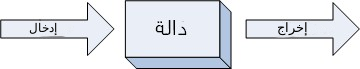
\includegraphics[width=0.8\textwidth]{Chapter_I-9_function-io}
\end{figure}

حينما نقوم باستدعاء دالة، نمرّ بثلاثة خطوات.

\begin{enumerate}
	\item \textbf{الإدخال}
	: نقوم بإدخال المعلومات إلى الدالة (بإعطائها معلومات تعمل عليها).
	\item \textbf{الحسابات}
	: تقوم الدالة بعمل حسابات على المعلومات التي تم ادخالها.
	\item \textbf{الإخراج}
	: بعد أن تنتهي الدالة من الحسابات تعطينا النتيجة على شكل قيمة الإخراج أو الإرجاع.
\end{enumerate}

يمكن أن نتصوّر دالة تسمى
\InlineCode{triple}
تضرب العدد في 3. بالطبع الدوال في الغالب هي أكثر تعقيداً من هذا.

\begin{figure}[H]
	\centering
	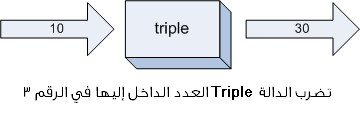
\includegraphics[width=0.8\textwidth]{Chapter_I-9_triple-io}
\end{figure}

هدف الدوال إذا هو تبسيط الشفرة المصدرية، لكي لا نضطر إلى إعادة كتابة نفس الشفرة المصدرية عدّة مرات على التوالي.

أُحْلُم قليلاً : لاحقاً، سننشئ مثلا دالة اسمها
\InlineCode{showWindow}
تقوم بفتح نافذة في الشاشة. ما إن نكتب الدالة (المرحلة الأصعب)، لن يتبقّ لنا سوى القول "أيتها الدالة
\InlineCode{showWindow}،
أظهري لي النافذة !". يمكننا أيضاً كتابة دالة
\InlineCode{moveCharacter}
تهدف إلى تحريك شخصية ما في اللعبة، إلخ.

\subsection{مخطط دالة}

لقد تكوّنت لديك فكرة على الطريقة التي تعمل بها الدالة 
\InlineCode{main}.\\
و مع ذلك يجب أن أريك كيف نقوم بإنشاء دالة. 

الشفرة المصدرية التالية تمثّل دالة تخطيطياً. هذا نموذج للحفظ :

\begin{Csource}
type functionName(parameters)
{
	// We write the instructions here
}
\end{Csource}

أنت تعرف شكل الدالة
\InlineCode{main}.\\
إليك ما عليك فهمه بخصوص المخطط.

\begin{itemize}
	\item \InlineCode{type}
	 (نوع قيمة الإخراج) : 
	هو نوع الدالة. مثل المتغيرات، للدوال أنواعها الخاصة. هذا النوع يعتمد على القيمة التي ترجعها الدالة : إن كانت الدالة ترجع عدداً عشرياً، فسنضع بالتأكيد الكلمة المفتاحية 
	\InlineCode{double}،
	أما إن كانت ترجع عدداً صحيحاً، سنضع النوع 
	\InlineCode{int}
	أو 
	\InlineCode{long}
	مثلا. و لكن يمكن أيضاً إنشاء دوال لا ترجع أي شيء !
	هناك إذا نوعان من الدوال :
	\begin{itemize}
		\item دوال ترجع قيمة : تعطيها أحد الأنواع الّتي نعرفها كـ\InlineCode{int}
		أو 
		\InlineCode{char}
		أو 
		\InlineCode{double}،
		إلخ.
		\item دوال لا ترجع أية قيمة : نعطيها نوعا خاصا يدعى 
		\InlineCode{void}
		(و الذي يعني الفراغ).
		\item \InlineCode{functionName} :
		هو اسم الدالة. يمكنك أن تسمي الدالة مثلما تريد لطالما تحترم القواعد التي تتبعها في تسمية المتغيرات (لا للأحرف التي تحتوي على العلامات الصوتية
		(\textenglish{accents})،
		لا فراغات، إلخ).
		\item \InlineCode{parameters} :
		(هي قيم الإدخال) : داخل قوسين، يمكنك أن تبعث معاملات للدالة. هي القيم التي ستعمل بها الدالة.
		\begin{information}
			يمكنك أن تبعث القدر الذي تريد من المعاملات. كما يمكنك ألا تبعث أية معامل، و لكن نادراً ما يُستخدم هذا.
		\end{information}
		
		مثلاً، بالنسبة للدالة 
		\InlineCode{triple}،
		أنت تبعث عدداً كمعامل. الدالة "تسترجع" العدد و تضربه في 3. تقوم بعد ذلك بإرجاع نتيجة حساباتها.
		\item بعد ذلك، نجد 
		\textbf{الحاضنتين}
		اللّتان تشيران إلى بداية الدالة و نهايتها. داخل الحاضنتين، تضع التعليمات التي تريدها. بالنسبة للدالة 
		\InlineCode{triple}،
		يجب أن تكتب التعليمات التي توافق ضرب قيمة الإدخال في 3.
	\end{itemize}
\end{itemize}
الدالة إذا هي عبارة عن آلية تتلقّى قيم إدخال (المعاملات) و ترجع قيمة إخراج.

\subsection{إنشاء دالة}

فلنرى مثالا تطبيقيّا دون مزيد من التأخير : الدالة 
\InlineCode{triple}
التي حدثتك عنها منذ قليل. فلنقل أن هذه الدالة تتلقّى عدداً صحيحاً من نوع 
\InlineCode{int}
و أنها تُرجع عدداً صحيحاً أيضاً من نوع 
\InlineCode{int}.
هذه الدالة تضرب العدد الذي نعطيها في 3 :

\begin{Csource}
int triple (int number)
{
	int result = 0;
	result = number * 3; // We multiply the input number by 3
	return result; // We return the result as an output value
}
\end{Csource}

هاهي أول دالة لك ! شيء مهمّ للغاية : كما ترى، الدالة من نوع 
\InlineCode{int}.
فهي مجبرة على  أن ترجع قيمة من نوع
\InlineCode{int}.

داخل القوسين، نجد المتغيرات التي تتلقّاها الدالة. الدالة 
\InlineCode{triple}
تتلقّى متغيرا من نوع 
\InlineCode{int}
يسمى 
\InlineCode{number}.

السطر الذي يشير إلى أن الدالة تقوم بـ"إرجاع قيمة" هو السطر الذي يحتوي على الكلمة المفتاحية 
\InlineCode{return}.
هذا السطر يوجد في العادة في نهاية الدالة، بعد الحسابات.

\begin{Csource}
return result;
\end{Csource}

هذه الشفرة المصدرية تعني للدالة : "توقّفي و أرجعي العدد 
\InlineCode{result}".
\underline{يجب أن}
يكون هذا المتغير
\InlineCode{result}
من نوع
\InlineCode{int}،
لأن الدالة تقوم بإرجاع قيمة من نوع
\InlineCode{int}
كما قلت في الأعلى.

صرّحت عن (= أنشأت) المتغير 
\InlineCode{result}
في الدالة 
\InlineCode{triple}.
هذا يعني أنه لا يستخدم إلا داخل هذه الدالة و ليس داخل أخرى كالـدالة
\InlineCode{main}
مثلا. أي أنه متغير خاص بالدالة 
\InlineCode{triple}.

لكن هل هذه هي الطريقة الأقصر لكتابة الدالة
\InlineCode{triple} ؟\\
لا، يمكننا كتابة محتوى الدالة في سطر واحد كالتالي :

\begin{Csource}
int triple (int number)
{
	return number * 3;
}
\end{Csource}

هذه الدالة تقوم بنفس المهمة التي تقوم بها الدالة السابقة، هي فقط أسرع من ناحية كتابتها. عموماً، الدوال التي تكتبها تحتوي الكثير من المتغيرات من أجل إجراء الحسابات عليها، نادرة هي الدوال القصيرة مثل
\InlineCode{triple}.

\subsection{العديد من المعاملات، لا معاملات}

\subsubsection{العديد من المعاملات}

الدالة
\InlineCode{triple}
تحوي معاملاً واحد، لكن من الممكن إنشاء دوال تقبل العديد من المعاملات.\\
مثلا، دالة 
\InlineCode{addition}
لجمع عددين
\InlineCode{a}
و 
\InlineCode{b} :

\begin{Csource}
int addition (int a, int b)
{
	return a + b;
}
\end{Csource}

يكفي تفريق المعاملات بفاصلة كما ترى.

\subsubsection{لا معاملات}

بعض الدوال، نادرة أكثر، لا تأخذ أية معامل كقيمة إدخال. هذه الدوال تقوم بنفس الشيء في غالب الأحيان. في الواقع، إذا لم تكن لديها أعداد تعمل عليها، فمهمة هذه الدوال هي القيام بوظائف معينة، كإظهار رسالة على الشاشة. و أيضاً، سيكون نفس النص الذي تظهره في كلّ مرة لأن الدالة لا تتلقّى أيّ معامل قد يكون قادرا على تغيير سلوكها !

تخيل دالة
\InlineCode{hello}
تقوم بإظهار الرسالة
"\textenglish{Hello}"
على الشاشة:

\begin{Csource}
void hello ()
{
	printf("Hello");
}
\end{Csource}

لم أضع أي شيء داخل الأقواس لأن الدالة لا تتلقّى أي معامل.\\
بالإضافة إلى ذلك، استعملت النوع 
\InlineCode{void}
الذي كلّمتك عنه أعلاه.

بالفعل، كما ترى فالدالة لا تحتاج إلى التعليمة 
\InlineCode{return}
لأنها لا ترجع أي شيء. الدالة التي لا ترجع أي شيء هي دالة من النوع
\InlineCode{void}.

\subsection{استدعاء دالة}

سنقوم الآن بتجريب الشفرة المصدرية للتمرّن قليلاً مع ما تعلّمناه.\\
سنستعمل الدالة 
\InlineCode{triple}
لضرب عدد في 3.

لحد الآن، أطلب منك كتابة الدالة 
\InlineCode{triple}
\underline{قبل}
الدالة 
\InlineCode{main}.
فإذا وضعتها بعدها، فلن يشتغل البرنامج. سأشرح لك هذا لاحقاً.

إليك الشفرة المصدرية التالية :

\begin{Csource}
#include <stdio.h>
#include <stdlib.h>
int triple(int number)
{
	return 3 * number;
}   
int main(int argc, char *argv[])
{
	int inputNumber = 0, tripleNumber = 0;
	
	printf("Enter a number... ");
	scanf("%d", &inputNumber);
	
	tripleNumber = triple(inputNumber);
	printf("The number's triple = %d\n", tripleNumber);
	
	return 0;
}
\end{Csource}

يبدأ البرنامج بالدالة 
\InlineCode{main}
كما تعلم.\\
نطلب من المستعمل إدخال عدد. نبعث هذا العدد كإدخال للدالة 
\InlineCode{triple}،
ثم نسترجع النتيجة في المتغير 
\InlineCode{tripleNumber}.
أنظر بشكل خاص السطر التالي:

\begin{Csource}
tripleNumber = triple(inputNumber);
\end{Csource}

داخل القوسين، نبعث المتغير كمدخل للدالة 
\InlineCode{triple}،
إنه العدد الذي ستعمل به الدالة. هذه الدالة تقوم بإرجاع قيمة، هذه القيمة نسترجعها في المتغير 
\InlineCode{tripleNumber}.
نأمر إذا الحاسوب في هذا السطر : "اُطلب من الدالة 
\InlineCode{triple}
ضرب العدد
\InlineCode{inputNumber}
في 3 و تخزين النتيجة في المتغير 
\InlineCode{tripleNumber}".

\subsubsection{نفس الشرح على شكل مخطط}

ألازالت لديك صعوبات في فهم المبدأ الذي تعمل به الدالة ؟\\
لا تقلق ! أنا متأكد أنك ستفهم بالمخططات.

هذه الشفرة المصدرية التي تحتوي على تعليقات سَتُريك في أي ترتيب يتم تنفيذ التعليمات. إبدأ إذا بقراءة السطر المرقّم 1 ثم 2، إلخ (أعتقد أنك فهمت) :

\begin{Csource}
#include <stdio.h>
#include <stdlib.h>
int triple(int number) // 6
{
	return 3 * number; // 7
}   
int main(int argc, char *argv[]) // 1
{
	int inputNumber = 0, tripleNumber = 0; // 2
	
	printf("Enter a number... "); // 3
	scanf("%d", &inputNumber); // 4
	
	tripleNumber = triple(inputNumber); // 5
	printf("The number's triple = %d\n", tripleNumber); // 8
	
	return 0; // 9
}
\end{Csource}

إليك ما يحدث سطراً بسطر :

\begin{enumerate}
	\item يبدأ البرنامج من الدالة
	\InlineCode{main}.
	\item يقرأ التعليمات في الدالة واحدة تلو الأخرى بالترتيب.
	\item يقرأ التعليمة الخاصة بالدالة
	\InlineCode{printf}.
	\item يقرأ أيضاً التعليمة الخاصة بالدالة 
	\InlineCode{scanf}.
	\item يقرأ التعليمة
	\dots
	آه نحن نستدعي الدالة 
	\InlineCode{triple}،
	يجب إذا أن نقفز إلى أول سطر من محتوى هذه الدالة في الأعلى.
	\item نقفز إلى الدالة
	\InlineCode{triple}
	 ثم نقوم باسترجاع المعامل
	\InlineCode{number}.
	\item نقوم بالحسابات و ننتهي من الدالة. الكلمة المفتاحية 
	\InlineCode{return}
	تعني أن الدالة قد انتهت و تسمح بتحديد النتيجة التي سترجعها الدالة.
	\item نرجع للدالة 
	\InlineCode{main}
	إلى التعليمة الموالية.
	\item نصل إلى 
	\InlineCode{return}
	و منه تنتهي الدالة
	\InlineCode{main}
	و ينتهي البرنامج.
\end{enumerate}

إذا فهمت في أي ترتيب يتم تنفيذ التعليمات فيه، فقد فهمت المبدأ. الآن يجب أن تفهم بأن الدالة تستقبل معاملات كمداخل و ترجع قيمة كمخرج.

\begin{figure}[H]
	\centering
	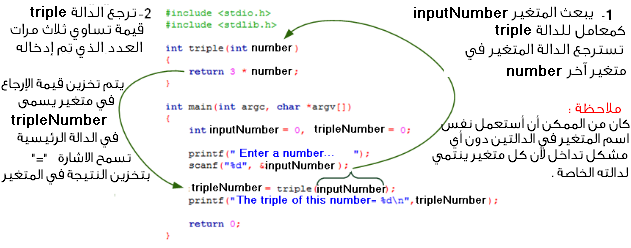
\includegraphics[width=\textwidth]{Chapter_I-9_triple-call}
\end{figure}

\paragraph{ملاحظة :}

ليس الأمر نفسه بالنسبة لكل الدوال. أحياناً، لا تأخذ الدالة أية معامل كإدخال، و بالعكس أحياناً تأخذ الكثير من المعاملات كإدخال (لقد شرحت لك هذا سابقاً).\\
أيضاً، يمكن لدالة أن ترجع قيمة كما يمكنها ألا ترجع أي شيء (و في هذه الحالة لا يكون هناك
\InlineCode{return}).

\subsubsection{فلنجرب هذا البرنامج}

هذا مثال عن تنفيذ البرنامج :

\begin{Console}
Enter a number... 10
The number's triple = 30
\end{Console}

\begin{information}
لست مضطراً إلى أن تخزن النتيجة في متغير ! يمكنك أن تعطي النتيجة المُرجعة من طرف الدالة 
\InlineCode{triple}
إلى دالة أخرى و كأن التعليمة
\InlineCode{triple(inputNumber)}
في حدّ ذاتها متغير.
\end{information}
لاحظ هذا جيداً، هي نفس الشفرة المصدرية لكن هناك تغيير آخر على مستوى 
\InlineCode{printf}.
بالإضافة إلى ذلك، لم نقم بالتصريح عن المتغير 
\InlineCode{tripleNumber}
و الذي لا يفيدنا في أي شيء الآن :

\begin{Csource}
#include <stdio.h>
#include <stdlib.h>
int triple(int number)
{
	return 3 * nombre;
}
int main(int argc, char *argv[])
{
	int inputNumber = 0, tripleNumber = 0و
	
	printf("Enter a number... ");
	scanf("%d", &inputNumber);
	// The result returned by the function is directly sent to printf without being saved in a variable
	printf("The number's triple = %d\n", triple(inputNumber));
	
	return 0;
}
\end{Csource}

كما ترى، استدعاء الدالة 
\InlineCode{triple}
يتم داخل الدالة 
\InlineCode{printf}.\\
ماذا يفعل الجهاز حينما يصل إلى هذا السطر من الشفرة المصدرية ؟

الأمر سهل، يجد أن السطر يبدأ بـ\InlineCode{printf}،
فسيقوم إذا باستدعاء الدالة 
\InlineCode{printf}.
يبعث إلى هذه الأخيرة كل المعاملات التي كتبناها. أول معامل هو النص الذي نريد طباعته و الثاني هو عدد.\\
يجد الجهاز بأنه قبل أن يبعث عددا إلى الدالة 
\InlineCode{printf}
عليه أولا استدعاء الدالة 
\InlineCode{triple}.
هذا ما يقوم به~: يستدعي 
\InlineCode{triple}،
يقوم بالحسابات و ما إن يتلقّ النتيجة حتّى يبعثها للدالة 
\InlineCode{printf} !

هذه الحالة تمثّل نوعاً ما تداخل الدوال. الشيء الذي نستنتجه من هذا هو أنه بإمكان دالة أن تستدعي دالة أخرى !\\
هذا هو مبدأ البرمجة بلغة
\textenglish{C} !
كلّ شيء مركّب مع الأشياء الأخرى، كما في لعبة
\textenglish{Lego}.

في النهاية، سيبقى الشيء الأصعب هو كتابة الدوال. ما إن تكتبها، لن يبق عليك سوى استدعائها دون أن تلقي بالا على العمليات التي تجري بداخلها. هذا سيسمح لك بتبسيط كتابة برامجك بشكل كبير. و صدّقني ستحتاج إلى هذه المبادئ كثيراً !

\section{أمثلة للفهم الجيّد}

كان عليك أن تلاحظ شيئاً : أنا شخص يلحّ كثيراً على الأمثلة.\\
المفاهيم النظرية مهمّة، لكنها لا تكفي لتذكّر كلّ شيء، كما أنك لن تفهم في أي شيء يمكنك استغلالها لاحقاً. و هذا سيكون أمرا مؤسفا.

سأريك إذا الآن عدة استعمالات للدوال لكي تأخذ فكرة عن أهميّتها. سأقدّم الكثير من الأمثلة المتخلفة محاولاً أن أعطيك لمحة عن كلّ أنواع الدوال التي يمكن أن توجد.

لن أعلّمك أي شيء جديد، لكنّه قد حان الوقت لرؤية أمثلة تطبيقية. إذا كنت قد فهمت ما سبق فهذا أمر جيّد و لن يعيقك أي مثال مما سيأتي.

\subsection{التحويل من الأورو الى الفرنك}

سنبدأ بدالة مشابهة كثيراً للدالة
\InlineCode{triple}،
لكنها تحمل أهمية لابأس بها هذه المرة : دالة تحوّل من الأورو إلى الفرنك. لمن لا يعرف فإن 1 أورو = 6,55957 فرنك.

سننشئ دالة نسميها 
\InlineCode{conversion}.\\
هذه الدالة تأخذ متغيرا كإدخال من نوع 
\InlineCode{double}
لأننا سنتعامل بالضرورة مع أعداد عشرية. إقرأها بتمعّن :

\begin{Csource}
double conversion(double euros)
{
	double francs = 0;
	francs = 6.55957*euros;
	return francs;
}
int main(int argc, char * argv[])
{
	printf("10 euros = %fF\n", conversion(10)); 
	printf("50 euros = %fF\n", conversion(50));
	printf("100 euros = %fF\n", conversion(100));
	printf("200 euros = %fF\n", conversion(200));
	return 0;
}
\end{Csource}

\begin{Console}
10 euros = 65.595700F
50 euros = 327.978500F
100 euros = 655.957000F
200 euros = 1311.914000F
\end{Console}

لا يوجد اختلاف كبير مقارنة بالدالة 
\InlineCode{triple}،
لقد أخبرتك بذلك مسبّقاً. الدالة 
\InlineCode{conversion}
طويلة قليلاً و يمكن أن يتم اختصارها في سطر واحد، سأترك لك عناء فعل ذلك بنفس الطريقة التي شرحتها لك مسبقاً.

في الدالة
\InlineCode{main}،
تعمّدت وضع الكثير من
\InlineCode{printf}
لأريك الهدف من استعمال الدوال. لكي أحصل على قيمة 50 أورو، ليس علي سوى استدعاء الدالة 
\InlineCode{conversion}
بإعطائها 50 كقيمة إدخال. و إذا أردت تحويل 100 أورو إلى الفرنك، كل ما أحتاج إلى فعله هو تغيير المعامل المرسل إلى الدالة (وضع القيمة 100 في مكان القيمة 50).

\paragraph{حان دورك !}
اكتب دالة ثانية (دائماً قبل الدالة 
\InlineCode{main})
تقوم بالعملية العكسية أي تحول من الفرنك إلى الأورو. لن يكون الأمر صعباً. هناك إشارة عملية تتغير ليس إلا.

\subsection{العقوبة}

سنهتم الآن بدالة لا تقوم بإرجاع أي شيء (لا وجود للإخراج).\\
هي دالة تقوم بإظهار نفس النص على الشاشة بالقدر الذي نحن نريد. هذه الدالة تأخذ كإدخال : عدد المرات التي نريد أن يظهر بها نص العقوبة على الشاشة.

\begin{Csource}
void punishment(int numberOfLines)
{
	int i;
	for (i=0; i<numberOfLines; i++){
		printf("I won't misbehave in class again\n");
	}
}
int main(int argc, char * argv[])
{
	punishment(10);
	return 0;
}
\end{Csource}

\begin{Console}
I won't misbehave in class again
I won't misbehave in class again
I won't misbehave in class again
I won't misbehave in class again
I won't misbehave in class again
I won't misbehave in class again
I won't misbehave in class again
I won't misbehave in class again
I won't misbehave in class again
I won't misbehave in class again
\end{Console}

هنا نتكلم عن دالة لا تُرجع أية قيمة. تكتفي هذه الدالة بالقيام بمهمة (هنا، إظهار النص على الشاشة).\\
الدالة التي لا ترجع أيه قيمة هي دالة من نوع 
\InlineCode{void}،
غير هذا لا يوجد شيء مختلف.

سيكون من الممتع أن نكتب دالة 
\InlineCode{punishment}
تتلائم مع أيّ عقوبة، فتقوم بإظهار النص الذي نريده نحن على الشاشة. نبعث لها معاملين : النص الذي نريد و عدد المرات التي نريد أن يتم إظهاره. المشكل هو أننا لا نجيد بعد التعامل مع النصوص في الـ\textenglish{C}
(إذا كنت لم تنتبه فأذكرك أنه لحدّ الآن لم نتعامل سوى مع متغيرات تحمل قيما عدديّة داخلها منذ بداية الكتاب !). و بهذا الصدد، أخبرك أننا لن نتأخر حتى نتعلّم كيفية التعامل مع النصوص. فعل ذلك معقّد قليلاً و لا يصلح أن نبدأ به في أول الكتاب !

\subsection{مساحة مستطيل}

من السهل حساب مساحة المستطيل : العرض $\times$ الطول.\\
الدالة التي سنكتبها
\InlineCode{rectangleSurface}
تأخذ معاملين : الطول و العرض. و تقوم بإرجاع المساحة.

\begin{Csource}
double rectangleSurface(double width, double height)
{
	return width * height;
}
int main(int argc, char * argv[])
{
	printf("Width = 5 and height = 10. Surface = %f\n", rectangleSurface(5,10));
	printf("Width = 2.5 and height = 3.5. Surface = %f\n", rectangleSurface(2.5,3.5));
	printf("Width = 4.2 and height = 9.7. Surface = %f\n", rectangleSurface(4.2,9.7));
	return 0;
}
\end{Csource}

\begin{Console}
Width = 5 and height = 10. Surface = 50.000000
Width = 2.5 and height = 3.5. Surface = 8.750000
Width = 4.2 and height = 9.7. Surface = 40.740000
\end{Console}

\begin{question}
هل يمكننا أن نظهر مباشرة طول، عرض و مساحة المستطيل داخل الدالة ؟
\end{question}

بالطبع ! في هذه الحالة لن ترجع الدالة أي شيء. ستكتفي بإظهار ما حسبته :

\begin{Csource}
void rectangleSurface(double width, double height)
{
	double surface;
	surface = width * height;
	printf("Width = %f and height = %f. Surface = %f\n", width, height, surface);
}
int main(int argc, char * argv[])
{
	rectangleSurface(5,10);
	rectangleSurface(2.5,3.5);
	rectangleSurface(4.2,9.7);
	return 0;
}
\end{Csource}

كما ترى، الـ\InlineCode{printf}
في
\textit{داخل}
الدالة
\InlineCode{rectangleSurface}
يعرض نفس الرسالة السابقة. هذه فقط طريقة مختلفة لفعل نفس الشيء.

\subsection{القائمة}

هذه الشفرة أكثر أهمية و واقعيّة. سننشئ دالة 
\InlineCode{menu}
لا تأخذ أي معامل كإدخال. تكتفي هذه الدالة بإظهار قائمة و تطلب من المستعمل اختيار ما يريد. الدالة تقوم بإرجاع اختيار المستعمل.

\begin{Csource}
int menu()
{
	int choice = 0;
	
	while (choice < 1 || choice > 4)
	{
		printf("Menu :\n");
		printf("1 : Royal Fried Rise\n");
		printf("2 : Noodle Basil \n");
		printf("3 : Pattaya Paradise \n");
		printf("4 : Spice Nitan Spicy...\n");
		printf("Your choice? ");
		scanf("%d", &choice);
	}   
	
	return choice;
}
int main(int argc, char * argv[])
{   
	switch (menu())
	{
		case 1:
		printf("You have chosen Royal Fried Rise\n");
		break;
		case 2:
		printf("You have chosen Noodle Basil \n");
		break;
		case 3:
		printf("You have chosen Pattaya Paradise \n");
		break;
		case 4:
		printf("You have chosen Spice Nitan Spicy\n");
		break;   
	}
	return 0;
}
\end{Csource}

اغتنمت الفرصة لتحسين القائمة (مقارنة بما نفعله عادة) : تقوم الدالة 
\InlineCode{menu}
بإظهار القائمة طالما لم يقم المستعمل بإدخال رقم محصور بين 1 و 4. فهكذا، لا يمكن أن تقوم الدالة بإرجاع قيمة لا تظهر على القائمة !

في الـ\InlineCode{main}،
تلاحظ أننا استعملنا 
\InlineCode{switch(menu())}.
بمجرّد أن تنتهي
\InlineCode{menu}،
فإنّها ستعيد خيار المستخدم مباشرة في
\InlineCode{switch}.
إنها طريقة سريعة و عمليّة.

\paragraph{حان دورك !}
يمكنك تحسين الشفرة المصدرية أكثر : يمكنك أن تظهر رسالة خطأ في حالة أخطأ المستعمل في الإختيار بدل أن تقوم بإعادة إظهار القائمة على الشاشة مرّة أخرى.

\section*{ملخّص}

\begin{itemize}
	\item يمكن لدالة أن تستدعي دالة أخرى. و لهذا فالـ\InlineCode{main}
	يمكنها استدعاء دوال جاهزة كـ\InlineCode{printf}
	و 
	\InlineCode{scanf}
	و كذلك دوالا ننشؤها بأنفسنا.
	\item تتلقّى الدالة كإدخال متغيّرات نسميها
	\textbf{معاملات}.
	\item تقوم الدالة ببعض العمليّات على هذه المعاملات و نُرجع عادة قيمة بالاستعانة بالتعليمة
	\InlineCode{return}.
\end{itemize}
